% ============================================================
%  孟凡腾 — 简历（风格 B · 学术简约／白纸细框）
%  数据与 cv_CN 一致，仅排版与视觉风格重做。
%  编译：xelatex cv_CN-academic.tex
% ============================================================
\documentclass[10.5pt,a4paper]{ctexart}

\usepackage[margin=1.85cm,top=1.6cm,bottom=1.6cm]{geometry}
\usepackage{xcolor}
\usepackage{graphicx}
\usepackage[colorlinks=true,linkcolor=ink,urlcolor=ink,hidelinks=false,pdftitle={孟凡腾 -- CV},pdfauthor={孟凡腾}]{hyperref}
\usepackage{enumitem}
\usepackage{setspace}

% ---- 调色板（学术冷调，克制）----
\definecolor{slateblue}{RGB}{47,93,143}     % 主色：蓝灰
\definecolor{ink}{RGB}{38,40,44}            % 正文墨色
\definecolor{muted}{RGB}{120,126,136}       % 弱灰文字
\definecolor{hair}{RGB}{208,214,223}        % 发丝线
\definecolor{hairdk}{RGB}{166,174,186}      % 略深发丝线
\definecolor{accentK}{RGB}{90,120,150}      % 楷体点缀

\linespread{1.06}

% ===================================================================
% 标题格式：白纸细框→ 无大色块，仅“细下划线＋左侧细竖线提示符”
% ===================================================================
\newcommand{\secbar}{\textcolor{hairdk}{\rule[0.35ex]{0.12em}{1.35em}}}

\newcommand{\cvsec}[1]{{%
  \par\noindent\nopagebreak\medskip
  \secbar\kern0.55em\textcolor{slateblue}{\sffamily\bfseries\large #1}\par\nopagebreak
  \noindent\textcolor{hair}{\rule[0.2em]{\textwidth}{0.55pt}}\par\nopagebreak
  \kern0.6em
}}

% 年份标签（细框虚化，不填充）
\newcommand{\greyyear}[1]{\textcolor{muted}{\sffamily\bfseries #1}}

% 亮点标签（发丝线细框，白底）
\newcommand{\subtlelabel}[1]{{\fcolorbox{hair}{white}{\kern1mm\footnotesize\sffamily\color{slateblue}#1\kern1mm}}}

% ===================================================================
% 页首：白纸 + 细线分隔 + 右上细框照片
% ===================================================================
\newcommand{\makecvheader}{%
  \noindent
  \begin{minipage}[t]{0.72\textwidth}
    \vspace{0.1em}
    {\fontsize{27}{31}\selectfont\sffamily\bfseries\color{ink}孟凡腾}
    \hspace{0.6em}{\large\color{muted}\mdseries Fanteng Meng}\\[3pt]
    {\color{accentK}\sffamily\mdseries 安全科学与工程 · 博士研究生}\\[7pt]
    {\small\color{ink}
     专长：无人机智能巡检 / 机器视觉 / 深度学习 \& 低空智能感知}\\[5pt]
    {\footnotesize\color{muted}北京交通大学 · 先进轨道交通自主运行全国重点实验室\\[1pt]
    交通运输学院（智能系）}
  \end{minipage}\hfill
  \begin{minipage}[t]{0.25\textwidth}
    \raggedleft
    \fcolorbox{hair}{white}{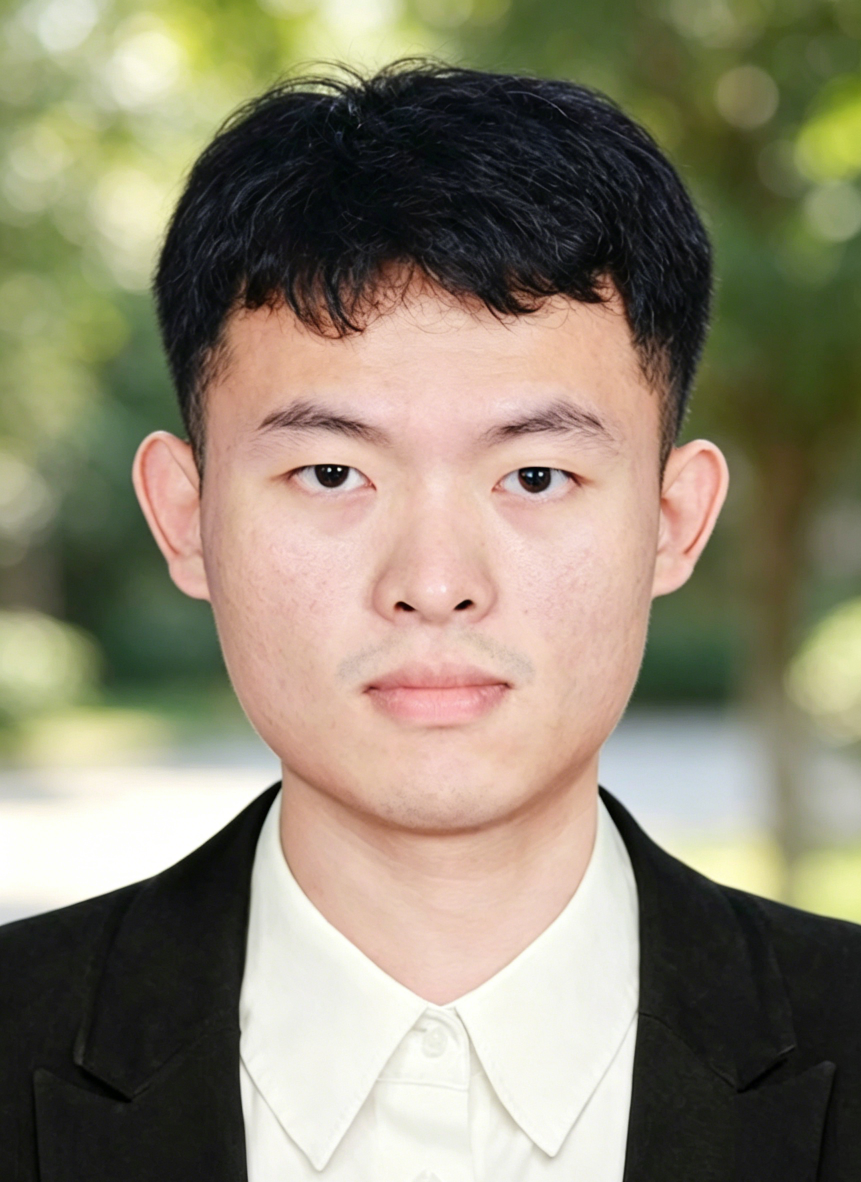
\includegraphics[width=2.55cm,height=2.55cm,keepaspectratio]{../images/photo-202601-square.png}}
  \end{minipage}
  \par\vspace{0.6em}
  \noindent\textcolor{hair}{\rule[0.2em]{\textwidth}{0.7pt}}\\[0.1em]
  \noindent{\scriptsize\sffamily\color{muted}
    \href{mailto:ftmeng@bjtu.edu.cn}{ftmeng@bjtu.edu.cn}\hspace{1.4em}$\cdot$\hspace{1.4em}
    \href{https://ft115.github.io}{ft115.github.io}\hspace{1.4em}$\cdot$\hspace{1.4em}
    \href{https://scholar.google.com.hk/citations?user=Yq5wnc8AAAAJ}{Google Scholar}}
  \\[0.2em]
  \noindent\textcolor{hair}{\rule[0.2em]{\textwidth}{0.7pt}}
  \vspace{0.6em}\par
}

\begin{document}
\makecvheader

% ==================== 教育经历 ====================
\cvsec{教育经历}

\noindent\textbf{博士 安全科学与工程} \hspace{0.6em}\greyyear{2023 — 至今}\par
\smallskip
\noindent\begin{tabular}{@{}p{0.51\textwidth}p{0.46\textwidth}@{}}
  北京交通大学 · 先进轨道交通自主运行全国重点实验室 &
  交通运输学院（智能系）\\
\end{tabular}
\noindent\\
{\footnotesize\color{muted}导师：秦勇 教授 · 硕博连读}

\vspace{0.7em}
\noindent\textbf{硕士 交通运输规划与管理} \hspace{0.6em}\greyyear{2022 — 2023}\par
\smallskip
\noindent{\footnotesize 北京交通大学}

\vspace{0.7em}
\noindent\textbf{本科 交通运输} \hspace{0.6em}\greyyear{2018 — 2022}\par
\smallskip
\noindent{\footnotesize 石家庄铁道大学}

% ==================== 研究方向 ====================
\cvsec{研究方向}

\noindent
无人机智能巡检　·　轨道交通机器视觉与深度学习　·　边缘计算　·　三维重建与点云分析

% ==================== 代表性论文 ====================
\cvsec{代表性论文}

{\footnotesize\color{muted}* 通讯作者；\# 共同第一作者。}

\vspace{0.4em}
\begin{enumerate}[leftmargin=1.7em,itemsep=3.5pt,topsep=1pt,labelsep=0.5em]
  \item \textbf{Meng, F.}, Qin, Y.$^*$, Wu, Y.$^*$, et al.\ ``SRLF: Sparse Representation Learning Framework for Railroad Surrounding Potential Risk Perception Using UAV Imagery.'' \textit{IEEE Trans.\ Intell.\ Transp.\ Syst.}, 2025.\\
    {\footnotesize\itshape\color{muted}IEEE T-ITS · 中科院 1 区 TOP · 5 年 IF 10.403}

  \item \textbf{Meng, F.}, Qin, Y.$^*$, Wu, Y.$^*$, Shao, C., Yang, H., Jia, L.\ ``Automatic Risk Level Evaluation System for Potential Environmental Hazards along High-speed Railroad Using UAV Aerial Photograph.'' \textit{Expert Syst.\ Appl.}, 2025.\\
    {\footnotesize\itshape\color{muted}Expert Systems with Applications · 中科院 1 区 TOP · 5 年 IF 8.995}

  \item \textbf{Meng, F.}, Qin, Y.$^*$, Wu, Y.$^*$, Shao, C., Jia, L.\ ``A Subtle Defect Recognition Method for Catenary Fastener in High-speed Railroad Using Destruction and Reconstruction Learning.'' \textit{Adv.\ Eng.\ Inform.}, 2024.\\
    {\footnotesize\itshape\color{muted}Advanced Engineering Informatics · 中科院 1 区 TOP · 5 年 IF 11.204}

  \item Wu, Y.$^\#$, \textbf{Meng, F.}$^\#$, Qin, Y.$^*$, Qian, Y.$^*$, Xu, F., Jia, L.\ ``UAV Imagery Based Potential Safety Hazard Evaluation for High-speed Railroad Using Real-time Instance Segmentation.'' \textit{Adv.\ Eng.\ Inform.}, 2023.\\
    {\footnotesize\itshape\color{muted}Advanced Engineering Informatics · 中科院 1 区 TOP · 5 年 IF 11.204}

  \item Wu, Y.$^\#$, \textbf{Meng, F.}$^\#$, Qin, Y.$^*$, Qian, Y.$^*$, Liu, Z., Zhao, W.\ ``Automated Anomaly Detection of Catenary Split Pins Using Unsupervised Learning.'' \textit{Autom.\ Constr.}, 2024.\\
    {\footnotesize\itshape\color{muted}Automation in Construction · 中科院 1 区 TOP · 5 年 IF 13.598}

  \item \textbf{孟凡腾}，秦勇$^{*}$，崔京，等.\ ``铁路外部环境无人机图像未知风险检测方法.'' \textit{航空学报（Acta Aeronautica et Astronautica Sinica）}, 2025.\\
    {\footnotesize\itshape\color{muted}《航空学报》· 中文航空领域权威期刊 · 卓越行动计划 T1 · EI}

  \item 秦勇$^{*}$，\textbf{孟凡腾}$^{\#}$，张紫城，等.\ ``轨道交通基础设施自主无人机智能巡检体系框架及其技术发展综述.'' \textit{北京交通大学学报}, 2025.\\
    {\footnotesize\itshape\color{muted}《北京交通大学学报》· 北大核心 · CSCD}
\end{enumerate}

% ==================== 代表性工程实践 ====================
\cvsec{代表性工程实践}

\noindent\textbf{高速铁路全自动无人机智能巡检系统}\par
\vspace{0.2em}
\begin{itemize}[leftmargin=0.85em,itemsep=2.5pt,label=\textcolor{muted}{$\cdot$}]
  \item \textbf{国内外首套高速铁路无人机自主智能巡检系统，规模应用近百公里。}
  \item 国家重点研发计划核心研究人员；设计 3 项原创视觉算法（召回率 >96%）。
  \item 部署 6 架巡检无人机 + 4 套自动化机巢；较人工巡检效率提升 10 倍以上。
\end{itemize}

\vspace{0.5em}\noindent\textbf{青藏铁路桥梁与落石灾害无人机智能巡检}\par
\vspace{0.2em}
\begin{itemize}[leftmargin=0.85em,itemsep=2.5pt,label=\textcolor{muted}{$\cdot$}]
  \item \textbf{平均海拔 3000+ 米自主飞行巡检。}
  \item 全栈技术研发：自主飞行控制、摄影测量三维重建、点云分割。
  \item 多期点云配准与落石形变检测，服务高原铁路运营安全。
\end{itemize}

\vspace{0.5em}\noindent\textbf{铁路钢桁梁桥无人机全覆盖巡检与涂层缺陷评估}\par
\vspace{0.2em}
\begin{itemize}[leftmargin=0.85em,itemsep=2.5pt,label=\textcolor{muted}{$\cdot$}]
  \item \textbf{GNSS 拒止下大跨度铁路钢桥飞行巡检。}
  \item 设计覆盖桥顶、桥侧及复杂桥底区域的避障巡检航线。
  \item 端到端流程：涂层缺陷识别 → 量化分级 → 缺陷空间溯源。
\end{itemize}

% ==================== 专利 ====================
\cvsec{专利}

\noindent\textbf{已授权专利}\par
\vspace{0.2em}
\begin{enumerate}[leftmargin=1.7em,itemsep=2pt,labelsep=0.5em]
  \item Autonomous UAV Based Intelligent Inspection System for Equipment, Facilities, and the Environment along Railway Lines and Method Thereof.\ {\scriptsize\color{muted}（美国发明专利）}
  \item 基于无人机图像的铁路环境隐患识别与风险等级评估方法
  \item 用于卫星拒止下交通设施巡检的无人机航线生成方法
  \item 跨模态自适应匹配的激光雷达与相机的在线外参标定方法及系统
\end{enumerate}

\vspace{0.3em}\noindent\textbf{已公开专利申请}\par
\vspace{0.2em}
\begin{enumerate}[leftmargin=1.7em,itemsep=2pt,labelsep=0.5em,resume]
  \item 用于无人机遥感图像的铁路沿线环境未知风险识别方法
  \item 一种用于铁路接触网的开口销缺陷精细化识别方法
  \item 铁路钢桁架桥涂层锈蚀检测评估方法及系统
\end{enumerate}

% ==================== 荣誉与获奖 ====================
\cvsec{荣誉与获奖}

\begin{tabular}{@{}ll@{}}
\greyyear{2024} & 第十四届“挑战杯”中国大学生创业计划竞赛“一带一路”国际邀请赛 · 银奖\\[1.2pt]
\greyyear{2024} & “青创北京”首都大学生挑战杯创业计划竞赛 · 银奖\\[1.2pt]
\greyyear{2022} & 北京交通大学暑期深度学习训练营 · 二等奖\\[1.2pt]
\greyyear{2021} & 中国交通优秀学子 · 一等奖\\[1.2pt]
\greyyear{2021} & 第七届全国大学生工程训练综合能力竞赛 · 省级一等奖\\[1.2pt]
\greyyear{2021} & 省级三好学生\\[1.2pt]
\greyyear{2020} & 第十二届全国大学生数学竞赛 · 省级一等奖\\[1.2pt]
\greyyear{2020} & 第七届全国大学生物理竞赛 · 省级一等奖\\
\end{tabular}

% ==================== 学术服务 ====================
\cvsec{学术服务}

\noindent\textbf{期刊审稿人：}\ \textit{IEEE Trans.\ Intell.\ Transp.\ Syst.}~(T-ITS)、\textit{Adv.\ Eng.\ Inform.}~(AEI)、\textit{Expert Syst.\ Appl.}~(ESWA)

% ==================== 专业技能 ====================
\cvsec{专业技能}

\noindent
编程语言与框架：Python、C++、Matlab\ \ $|$\ \ 深度学习：PyTorch\ \ $|$\ \ 系统：Linux、ROS
\ \ $|$\ \ 视觉：OpenCV\ \ $|$\ \ 机载：DJI-PSDK

\end{document}
